% TODO BY FELIX

The following chapter will describe the graphical user interface of Voxie.

\subsection{Windows}

Voxie is an application built around one main window. It contains all main
features like showing visualizers and the runtime configuration in the
side panel.

\subsubsection{Main Window}

\begin{figure}[h]
	\caption{Main Window}
	\centering
	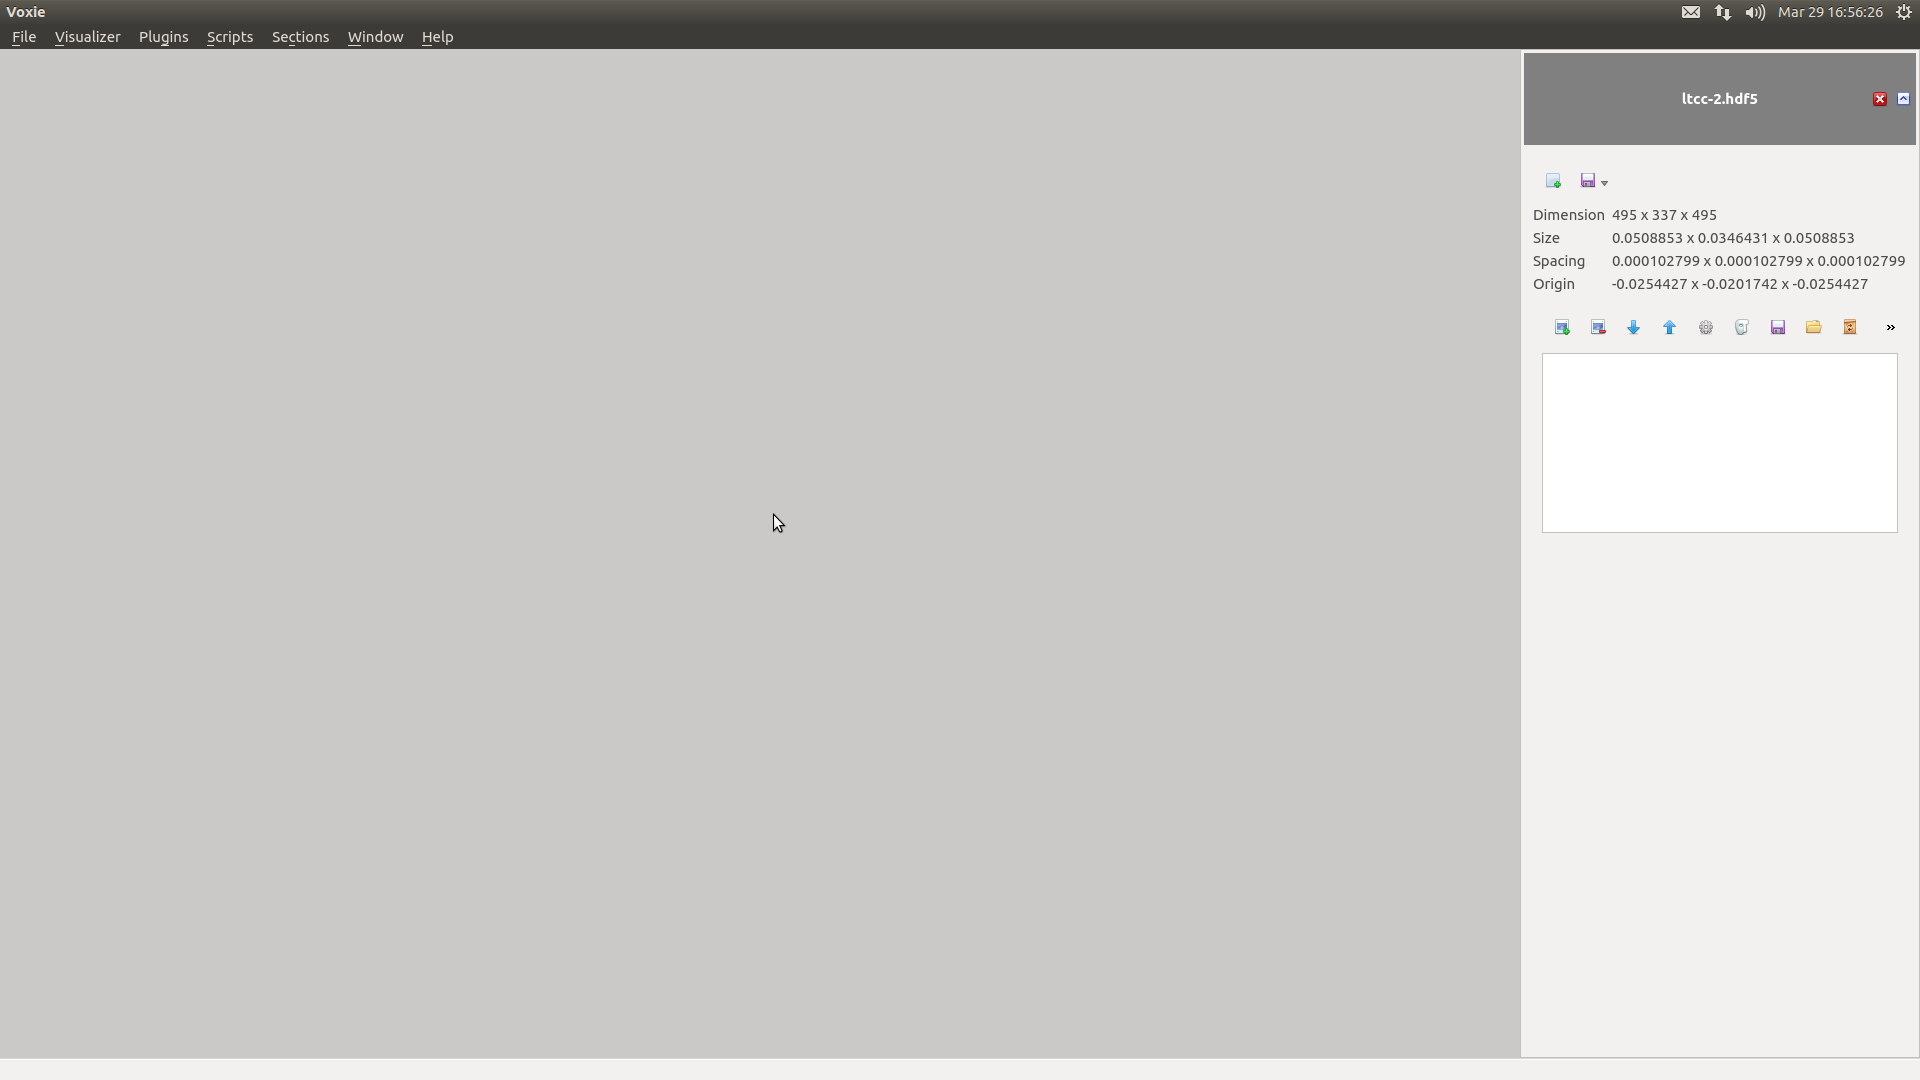
\includegraphics[width=1.0\textwidth]{img/mainwindow.png}
\end{figure}

The main window opens when Voxie gets started. It contains the main menu,
the side panel and shows all open visualizers in the center.

The side panel is described further in \ref{sections}.

The main menu is described futher in \ref{menus}.

\subsubsection{Preferences Window}
\label{preferences-window}

The preferences window allows the user to modify and customize Voxie for
his needs.

It allows setting up custom script types for external script files, select the
used OpenCL devices and options provided by plugins.

\begin{figure}[h]
	\caption{Preferences Window}
	\centering
	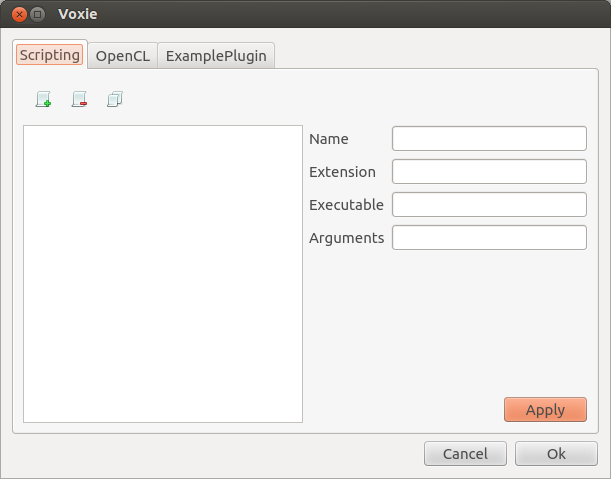
\includegraphics[width=0.6\textwidth]{img/preferences-script.png}
\end{figure}

\subsubsection{Scripting Window}
\label{scripting-window}

The scripting window provides a small JavaScript console for live scripting.
A line of code can be entered in the bottom text box and with a click on \emph{Run!}
or a on the return key, the script will be executed.
It is possible to navigate through previously executed commands by pressing the up or
down arrow key.

It also shows a live debug log from running scripts.

\begin{figure}[h]
	\caption{Scripting Window}
	\centering
	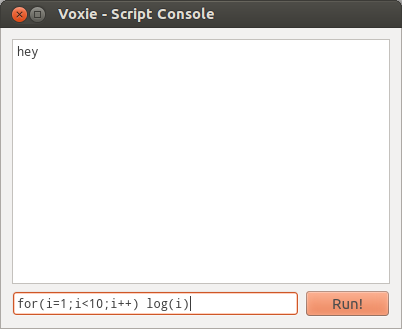
\includegraphics[width=0.5\textwidth]{img/script-console.png}
\end{figure}


\subsubsection{Visualizer Windows}

Visualizer windows are a special kind of window.
Each visualizer can be separated from the main window
as a standalone window.

Those visualizer windows behave like the integrated windows
except they can be positioned anywhere on the work space
(including other monitors).

Separating a window can be achieved by clicking the "Pop out" button
on top of each visualizer.

\subsection{Menus}
\label{menus}

\subsubsection{File}

The file menu contains the main control of Voxie as well as options to load
files.

To load a file, there are two options:
\begin{itemize}
	\item{Loading a file}
	\item{Using an importer}
\end{itemize}
Loading a file always shows a file dialog (Fig. \ref{file-dialog}) which allows selection of
all plugin supported file types. Most options show an additional dialog after
confirming the dialog to make further settings on opening the file.

Example:\newline
The HDF5 importer shows a dialog for selection of the dataset as can bee
seen in Fig. \ref{hdf5-dialog}.

Using importers allows a more flexible way of loading data sets.
Importers are not bound to any predefined procedures, they can show any
kind of UI and allow advanced loading of data sets, e.g. like loading a data
set from multiple files, reading a data set from an external device or 
even just create a data set on the fly.

The file menu also contains an option to quit Voxie and another to set up
preferences for Voxie itself as well as for plugins that support options.

\begin{figure}[h]
	\caption{File Dialog}
	\centering
	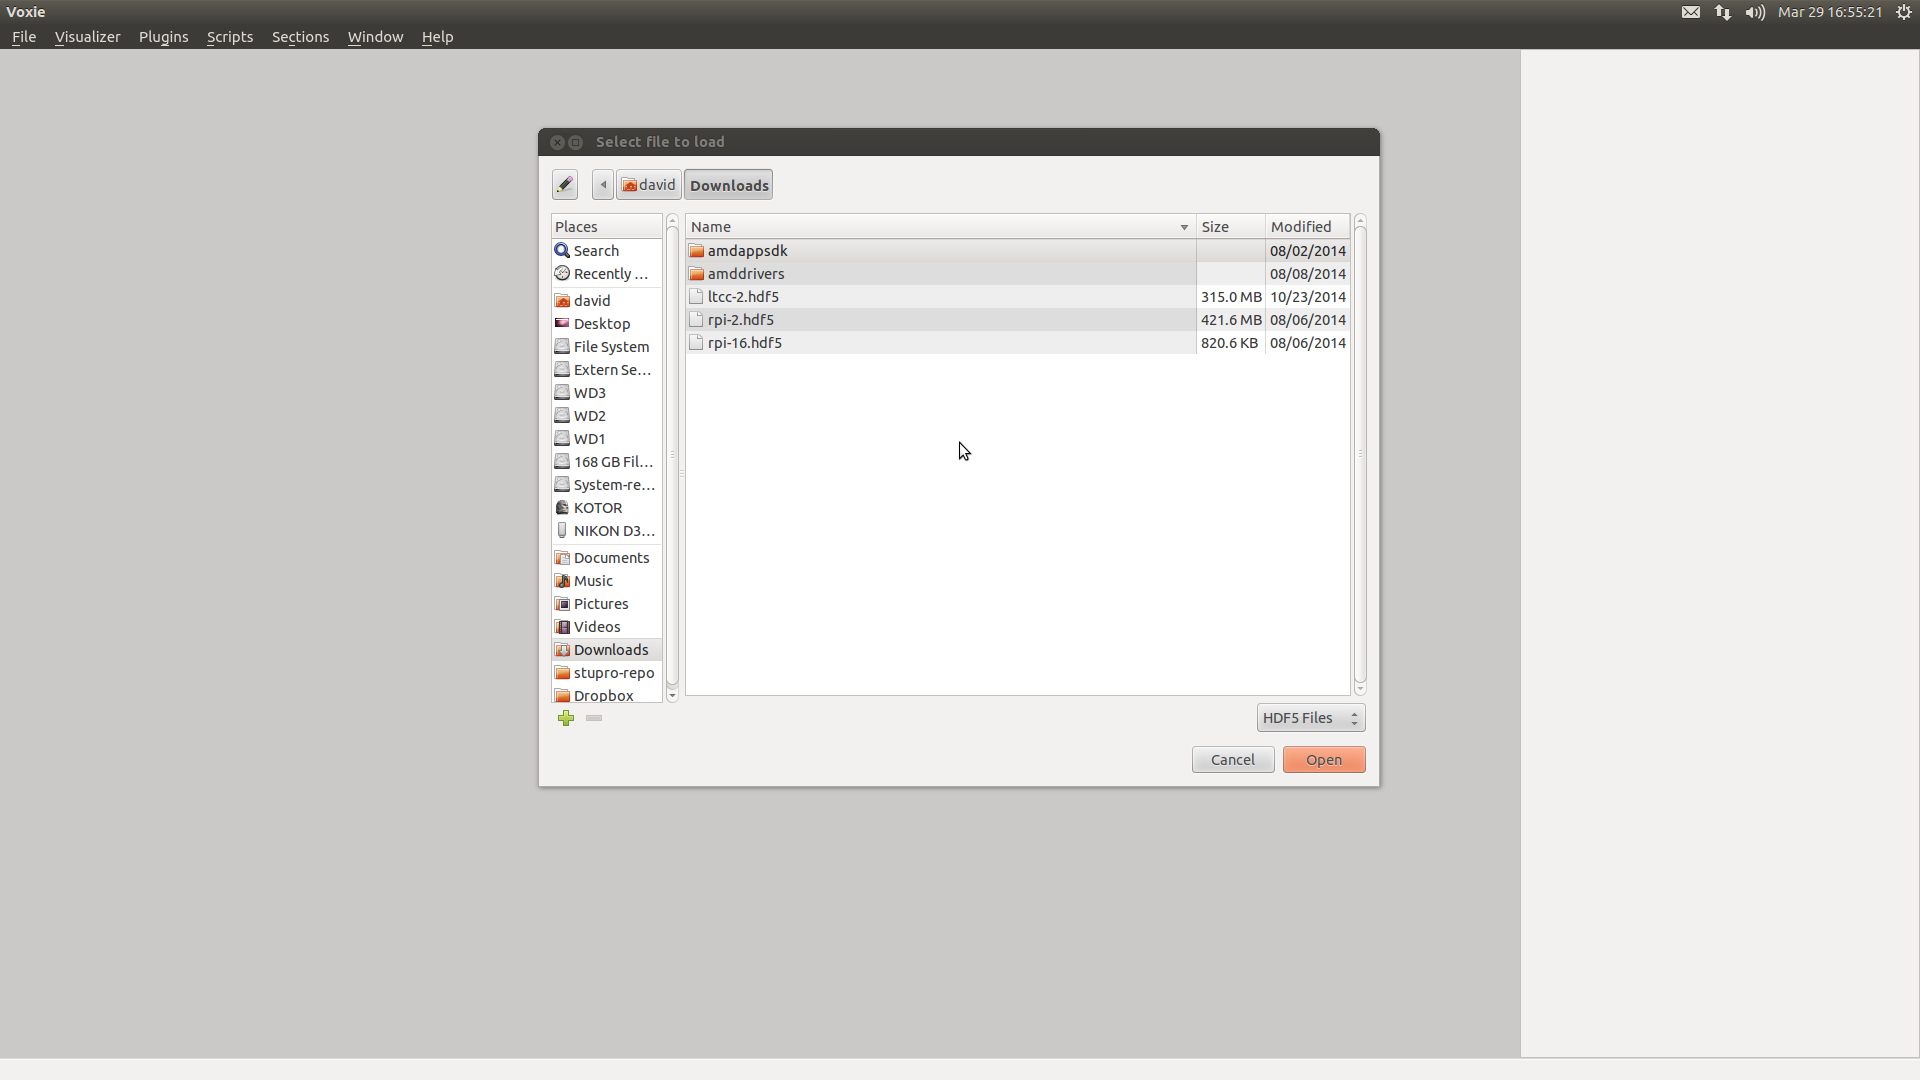
\includegraphics[width=1.0\textwidth]{img/file-dialog.png}
	\label{file-dialog}
\end{figure}

\begin{figure}[h]
	\caption{HDF5 Dialog}
	\centering
	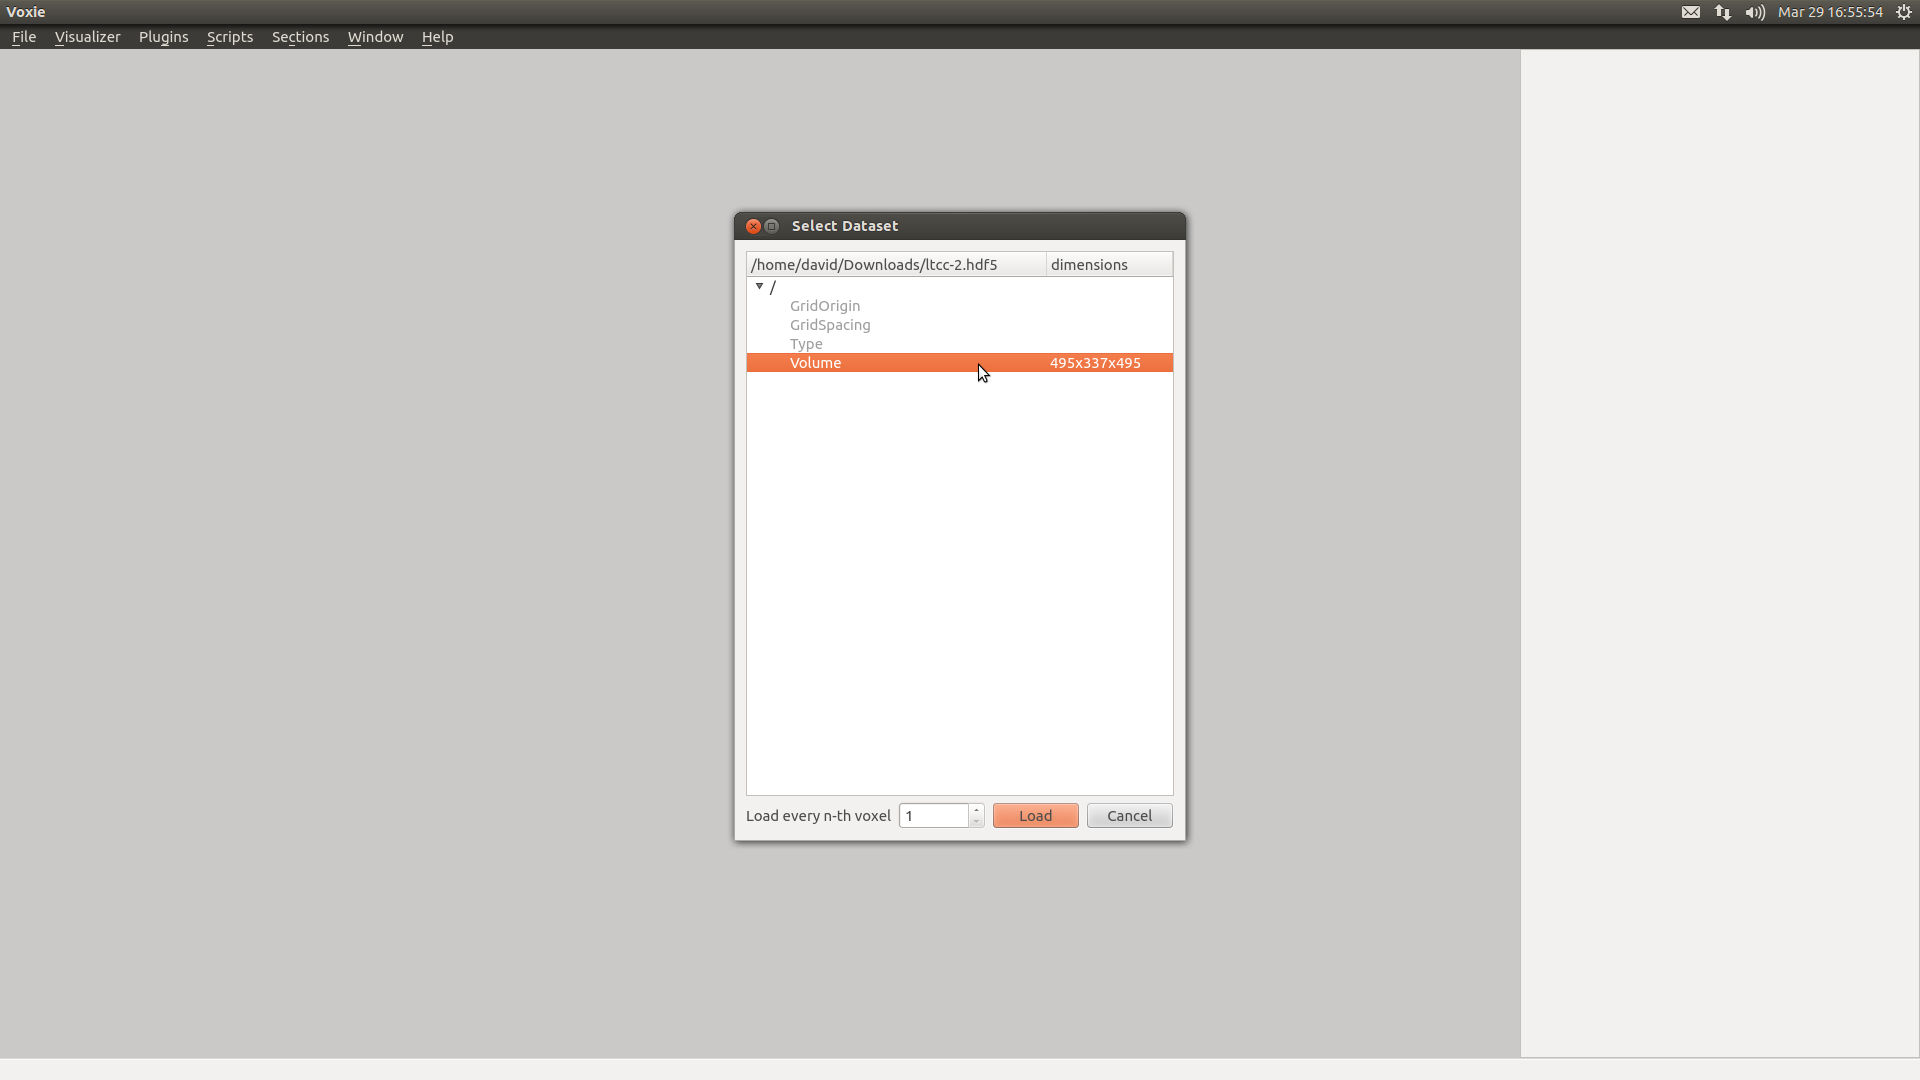
\includegraphics[width=1.0\textwidth]{img/hdf5-dialog.png}
	\label{hdf5-dialog}
\end{figure}


% Achso und dann noch hdf5 Datei laden

\subsubsection{Visualizer}

The visualizer menu contains sorted entries to create new visualizers.
Visualizers are ordered in 4 categories:
\begin{itemize}
	\item{\emph{2D} \newline Visualize voxel data in 2D.}
	\item{\emph{3D} \newline Visualize voxel data in 3D.}
	\item{\emph{Analytic} \newline Analyze the voxel data without a graphical visualization.}
	\item{\emph{Miscellaneous} \newline Every kind of visualizer that does not fit
		in the above categories }
\end{itemize}

\subsubsection{Plugins}

This menu shows an entry for each plugin that supports UI Commands (see \ref{ui-command}).
Each entry contains all UI commands for that plugin.

The UI command will be invoked by clicking the command entry.

\subsubsection{Scripts}

This menu allows to show the scripting console which is explained in \ref{scripting-window}.

It also shows all files that reside the folder \emph{scripts} next
to the voxie executable. A click on a script will execute it.

JavaScript (*.js) files are shown by default and will be executed by the
internal JavaScript scripting engine.

Other scripts can be configured to be shown in the menu by setting up a new
script type in the \emph{Scripting}-Section of the preferences window (See \ref{preferences-window}). The files will be executed by starting the external
application defined there.

\subsubsection{Sections}

The \emph{Sections} menu will show all currently active sections.
A click on the menu item will show or hide the section in the side panel.

\subsubsection{Windows}

This menu allows to reorder all currently opened visualizer windows in 4 styles:
\begin{itemize}
	\item{\emph{Cascade}\newline Will cascade the windows from the top left
		corder to the bottom right corner.}
	\item{\emph{Tile}\newline Will till the windows in a regular grid.}
	\item{\emph{Fill}\newline Will maximize the current window.}
	\item{\emph{Tabbed}\newline Will enable or disable tabbed mode. In tabbed mode,
		all windows are maximized and can be switched with a tab control.}
\end{itemize}

\begin{figure}[h]
	\centering
	\def\tabularxcolumn#1{m{#1}}
	\begin{tabularx}{\linewidth}{@{}cXX@{}}
		\begin{tabular}{cc}
			\subfloat[Cascade]{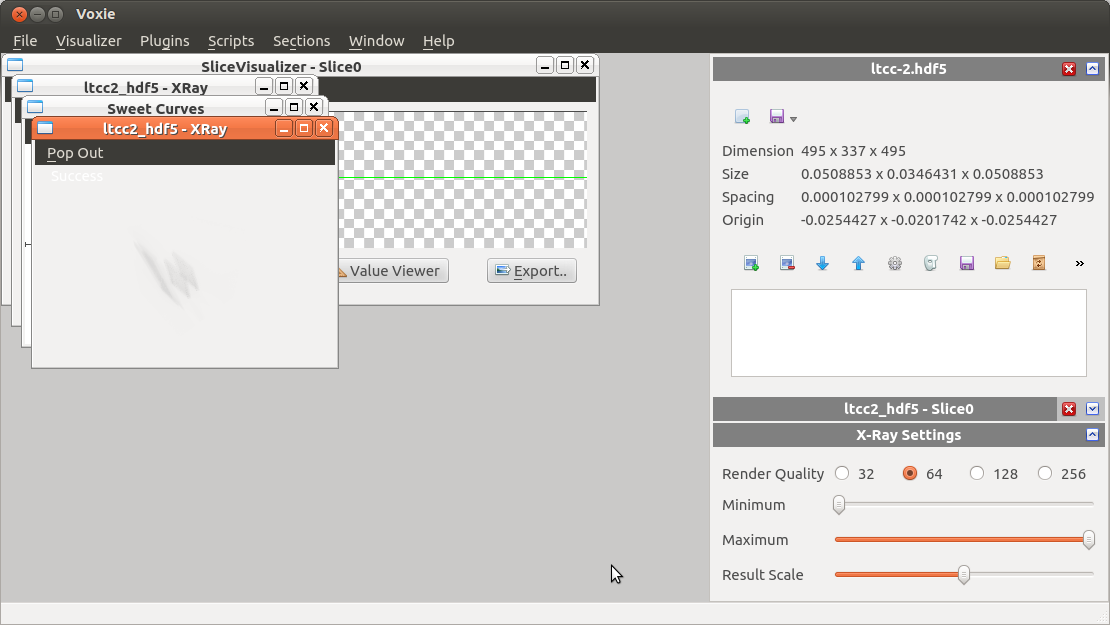
\includegraphics[width=0.5\textwidth]{img/window-cascade.png}} 
			& \subfloat[Tile]{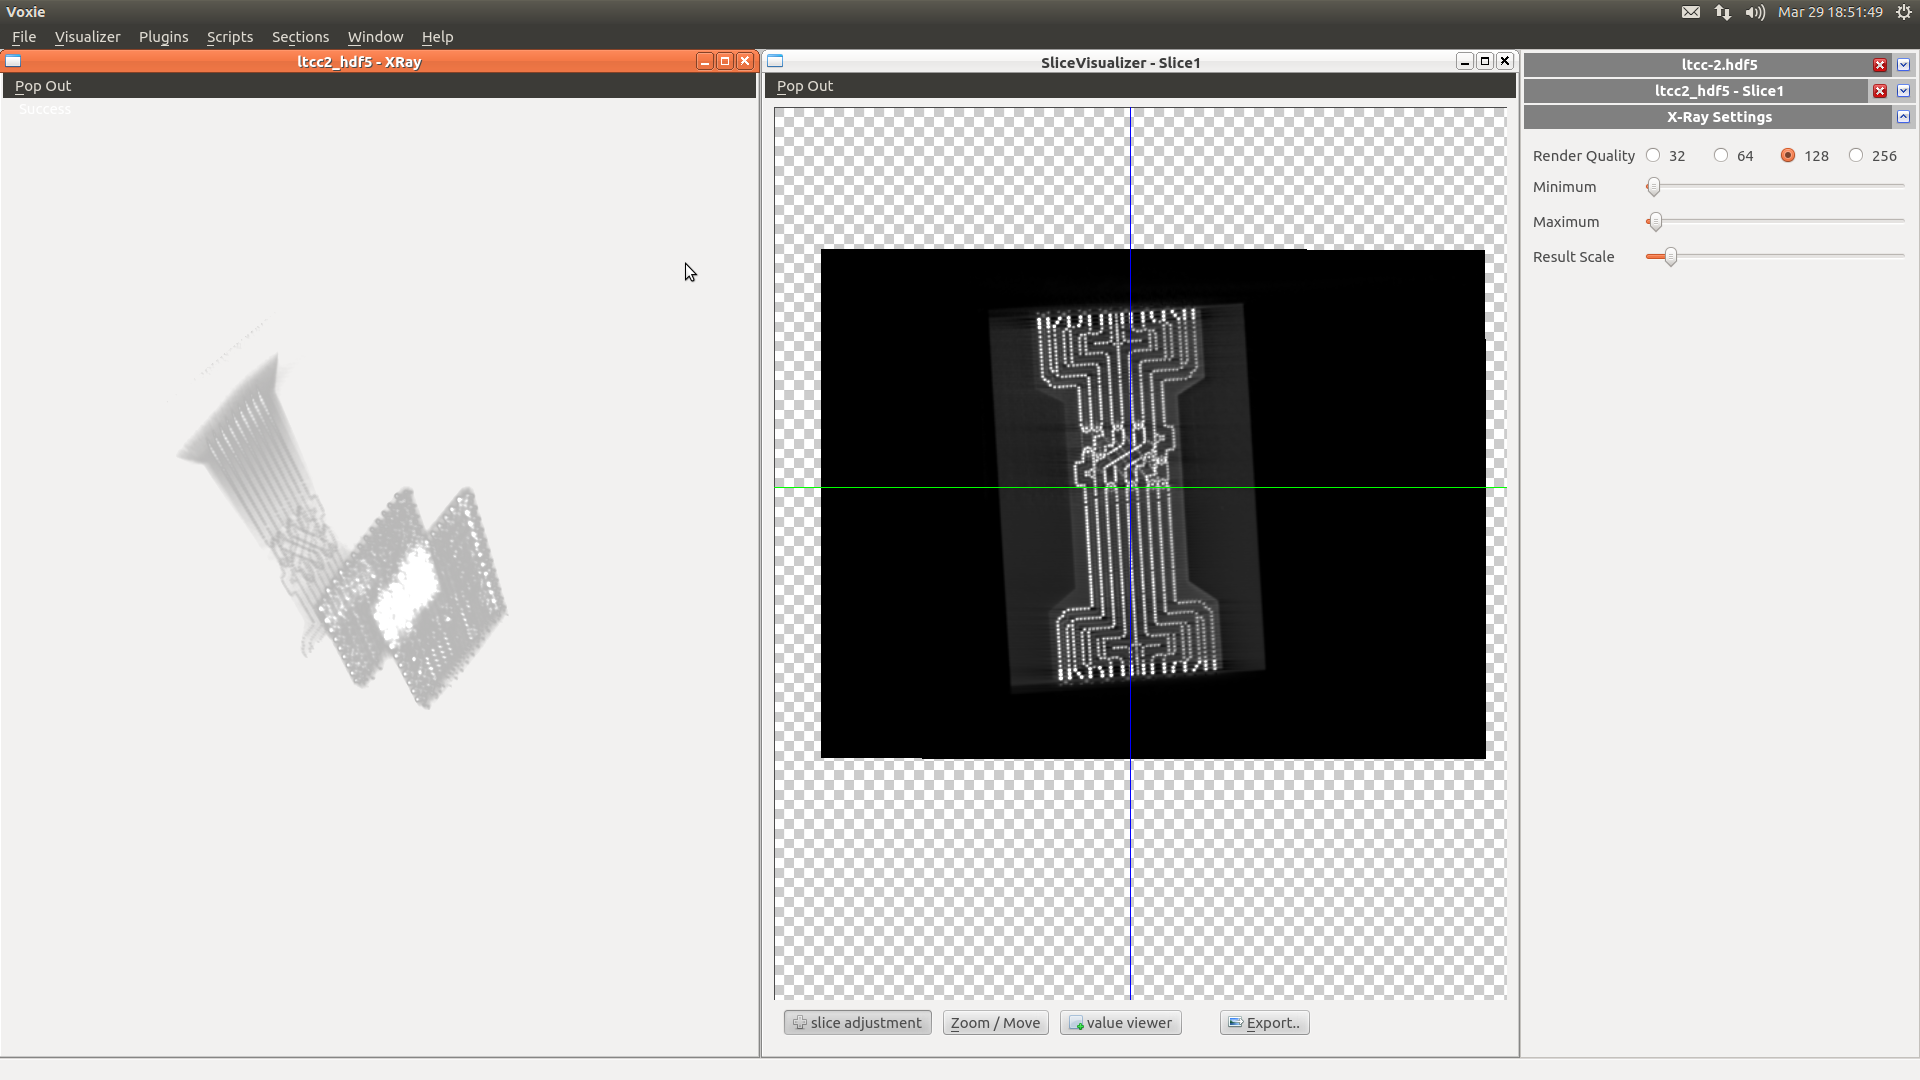
\includegraphics[width=0.5\textwidth]{img/window-tile.png}}\\
			\subfloat[Fill]{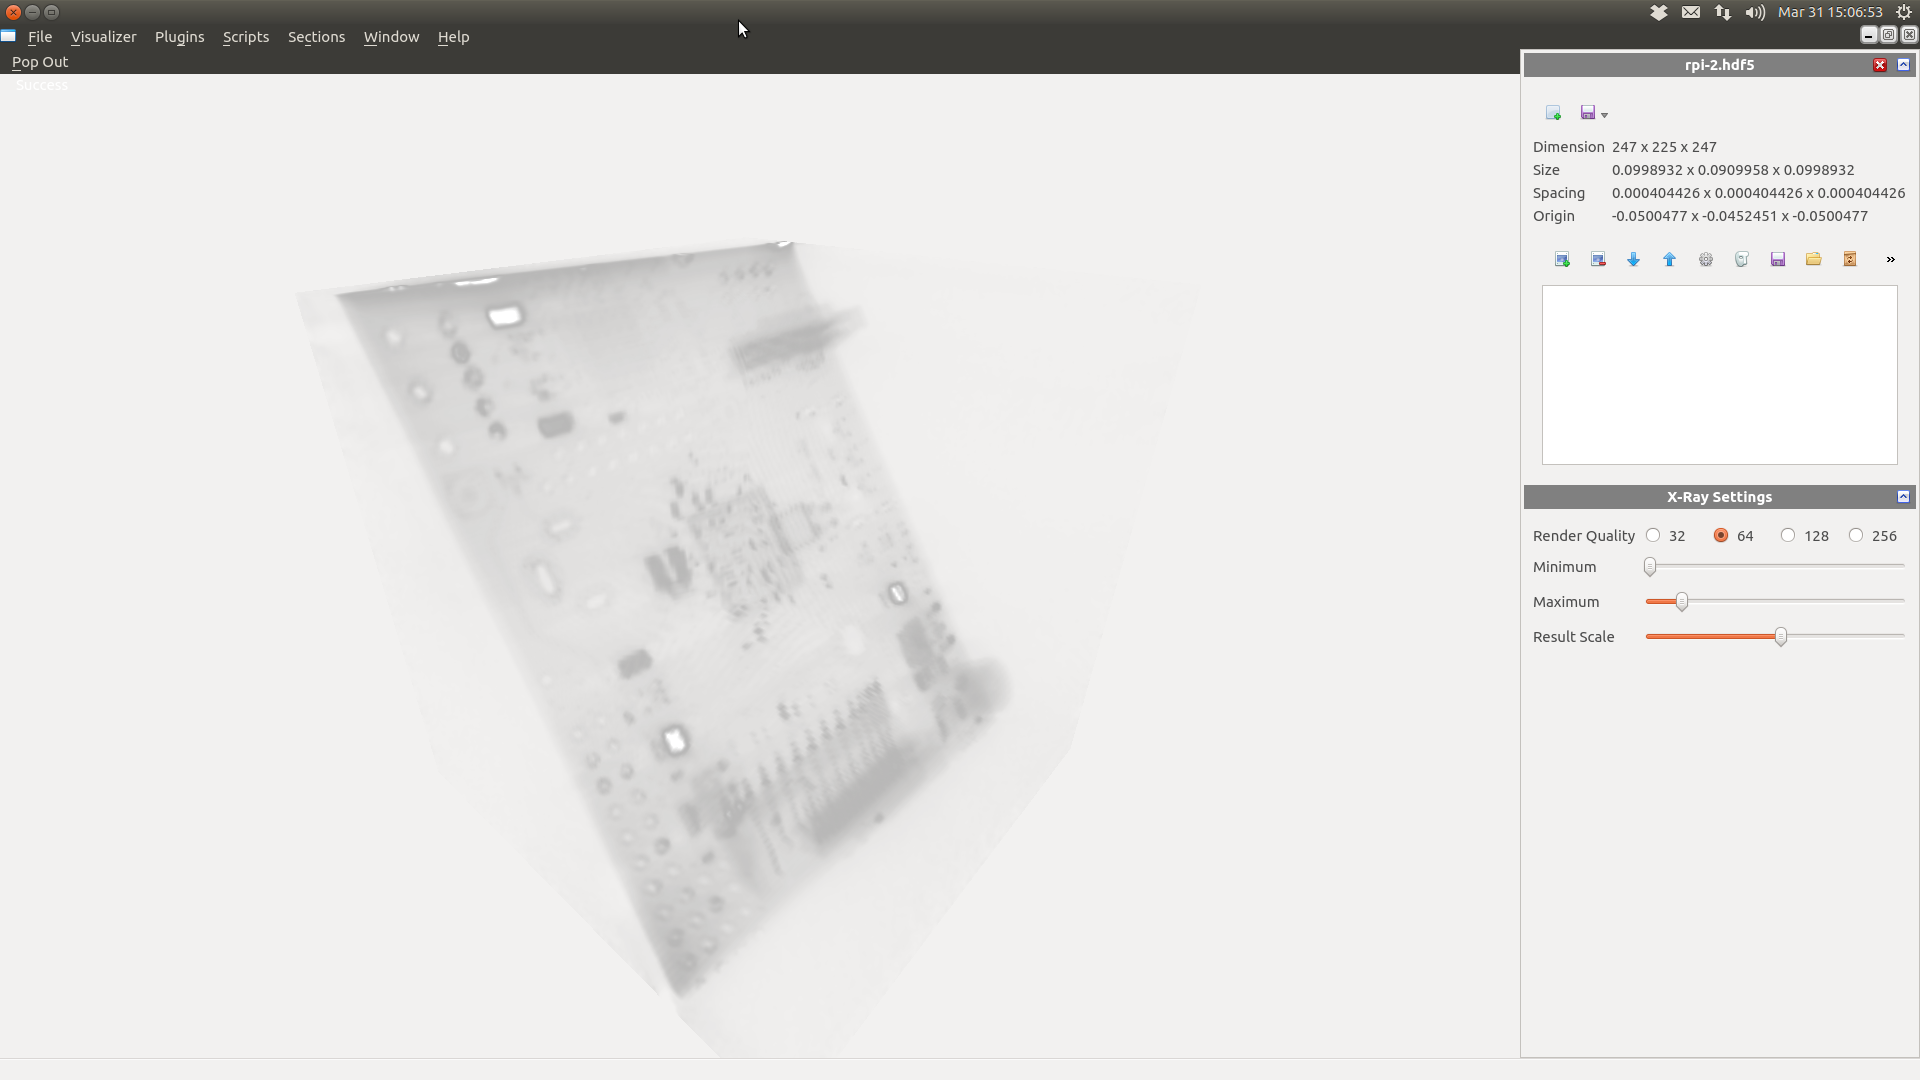
\includegraphics[width=0.5\textwidth]{img/window-fill.png}} 
			& \subfloat[Tabbed]{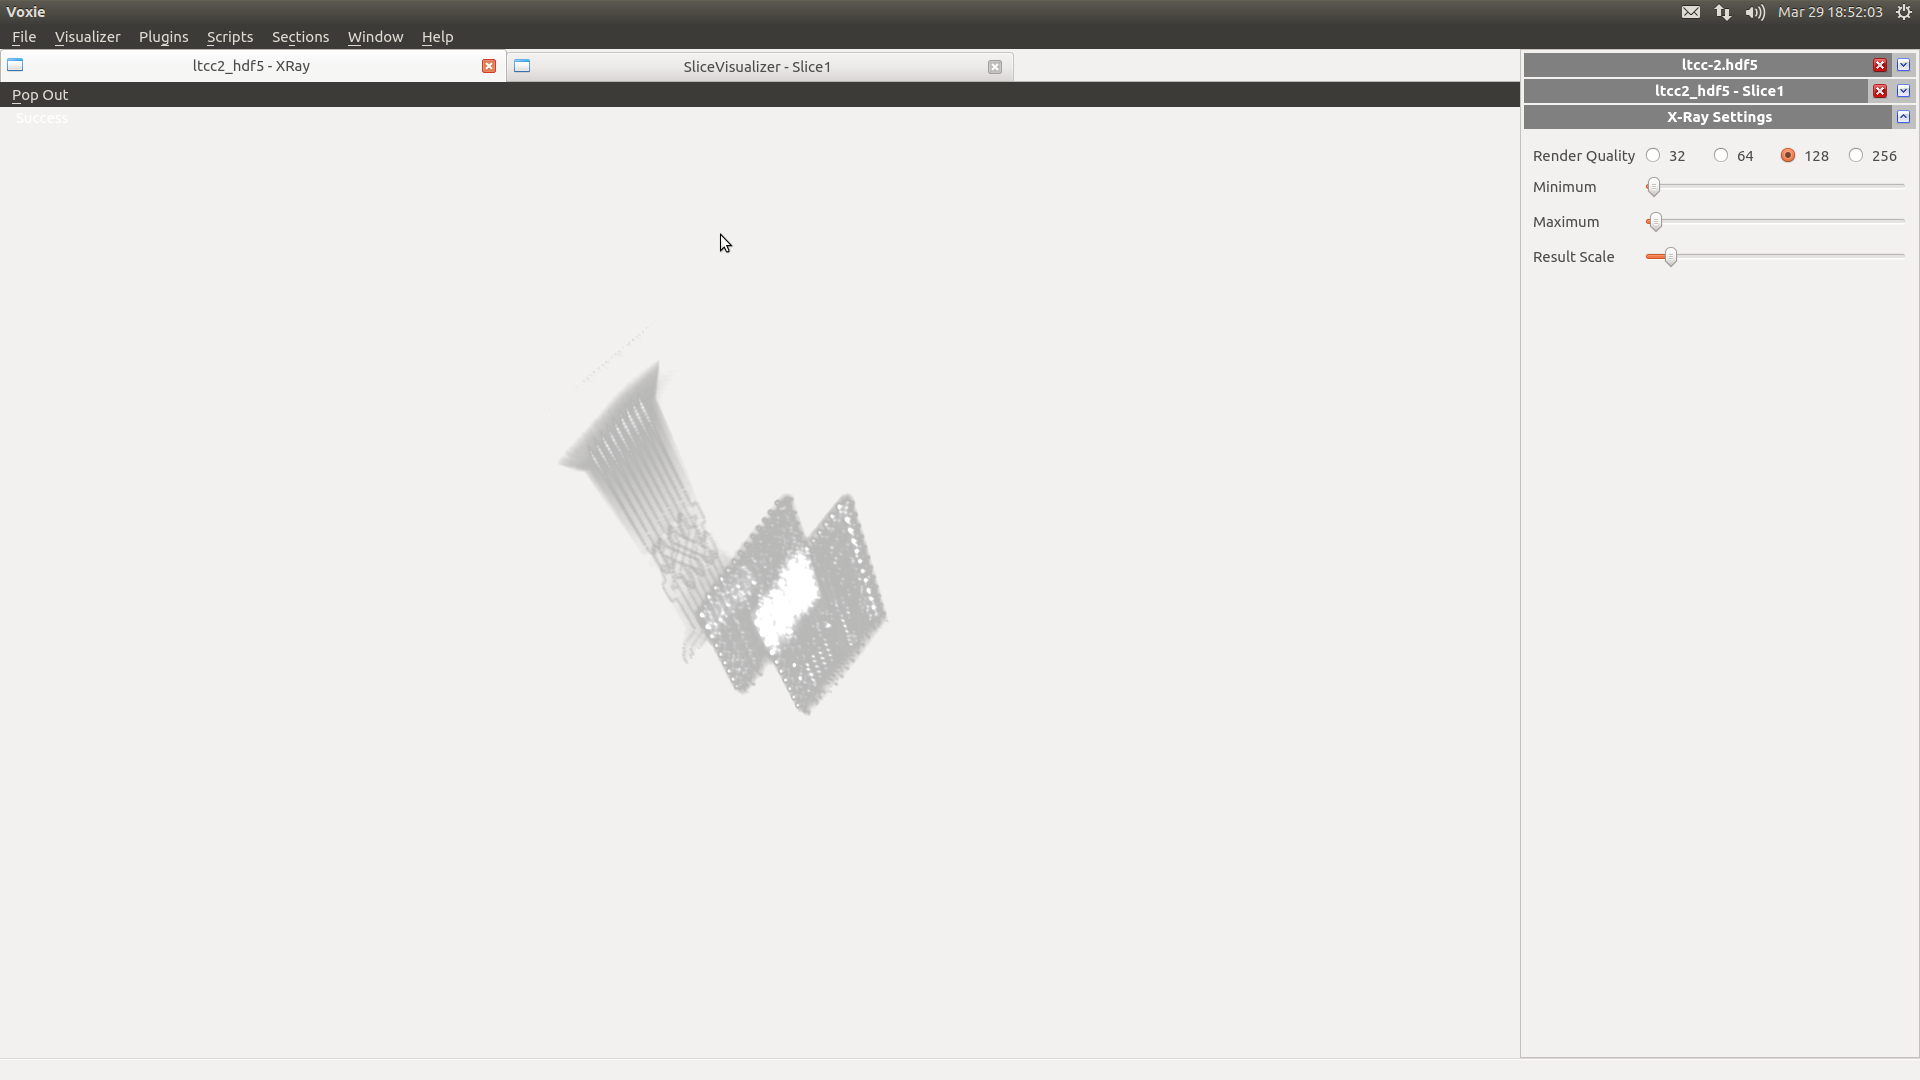
\includegraphics[width=0.5\textwidth]{img/window-tabbed.png}}\\
		\end{tabular}
	\end{tabularx}
	\caption{Window Modes}
	\label{windows-tile}
\end{figure}

\subsubsection{Help}

The help menu offers several possibilites to get help with Voxie:

\begin{itemize}
	\item{\emph{Manuel}\newline Opens this manual.}
	\item{\emph{Wiki}\newline Opens the wiki in the default browser.}
	\item{\emph{About}\newline Shows an about dialog with some quick info about Voxie.}
\end{itemize}

\subsection{Sections}
\label{sections}

Voxie features the side panel, a multifunctional panel showing context dependent
information and settings to the currently active data sets and visualizers.

Sections can be collapsed so they only show their header and may be closable.
If a section gets closed, all data connected will be released (e.g. closing
a data set will close all attached visualizers and slices as well).

% Nur generisch und dataset und slice section

\subsubsection{Data Set Section}
